% requires the hyperref package
% also requires graphicx

\section{The Control System}

This section describes the embedded control system and user interaction.
The latest system software and documentation can always be found on github at \url{https://github.com/hedj/fusion/}.

Flowcharts in this section use the visual language from the DRAKON project. See \url{http://drakon-editor.sourceforge.net/language.html} for details.

\begin{figure}
  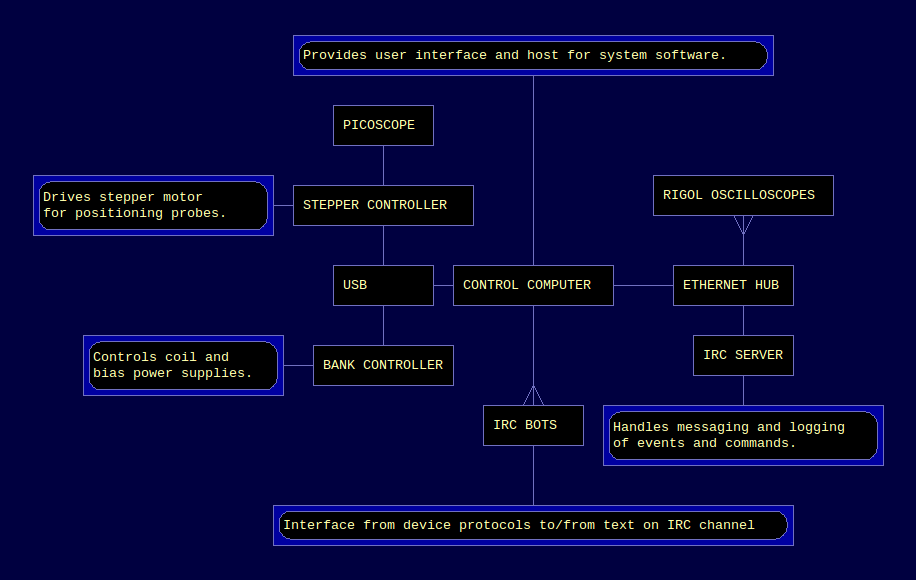
\includegraphics[width=400px]{system_structure.png}
\caption{\label{fig:system} Overall system design}
\end{figure}

\subsection{The Control Computer}

The control computer is a standard PC presently running Windows 10. It shares its connection to the
internet via ethernet, which is connected to a hub. Oscilloscopes and the IRC server hang off this hub.
At present, all the software agents described later run on the control computer, although in principle
it would be possible to run many of them on other computers.

\subsection{The Bank Controller}

The bank controller is a \href{http://controllino.biz/product/controllino-mega/}{Controllino Mega}; an
Arduino-based programmable-logic controller. The bank controller is in charge of the following functions:
\begin{itemize}
  \item{Capacitor-bank and HV pulse generation}
  \item{HV voltage control}
  \item{Capacitor bank charge control}
  \item{Audible alert before pulse}
\end{itemize}

The top-level flow of the bank controller is shown in Fig.~\ref{fig:toplevelbank}.

\begin{figure}
  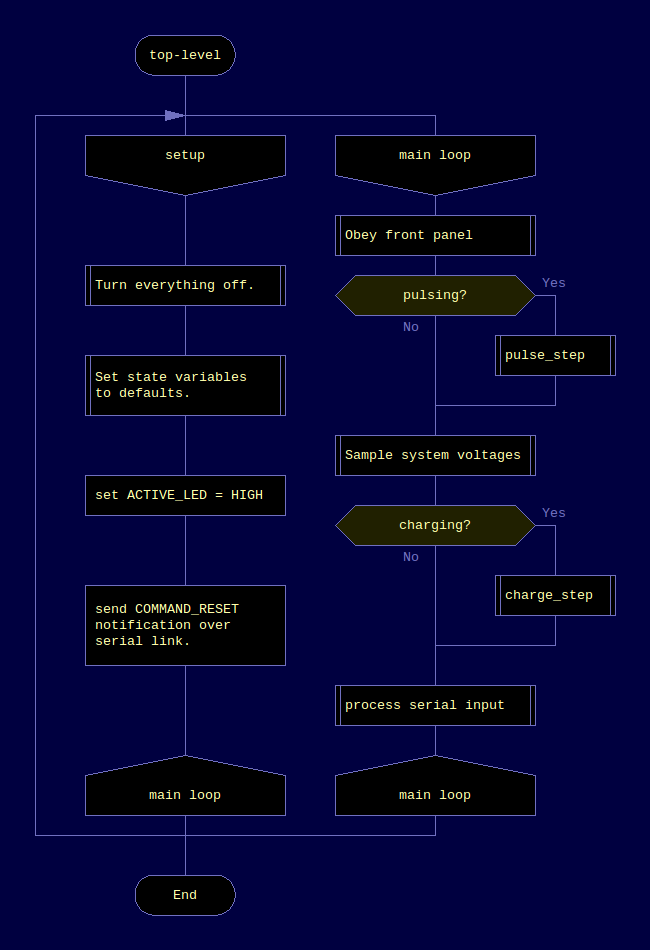
\includegraphics[width=400px]{top_level.png}
\caption{\label{fig:toplevelbank} Top-level flow of the bank controller}
\end{figure}

The serial protocol used is nonstandard; a definition can be found at \url{https://github.com/hedj/nslc}.  It is designed to facilitate debugging using a serial terminal; nslc is a simple frame-based protocol using line-feeds as end-of-frame markers and whitespace for escape. It is also checksummed for reliability. The particular checksum is only 8 bits in size, and is optimised for speed of implementation.

The most important thing to emphasise is that the controller is implemented as a tight loop reacting to the change in time. There are no blocking wait statements; in this way we ensure that input can continue to be received from the front panel switches or serial as the process runs. This allows the safe abort of the system regardless of its state, which is rather important.

The two operations which consume a reasonable amount of time and are thus implemented as conditional actions in the inner loop are pulsing and charging, respectively Figs.~\ref{fig:pulse_step}~and~\ref{fig:charge_step}.

\begin{figure}
  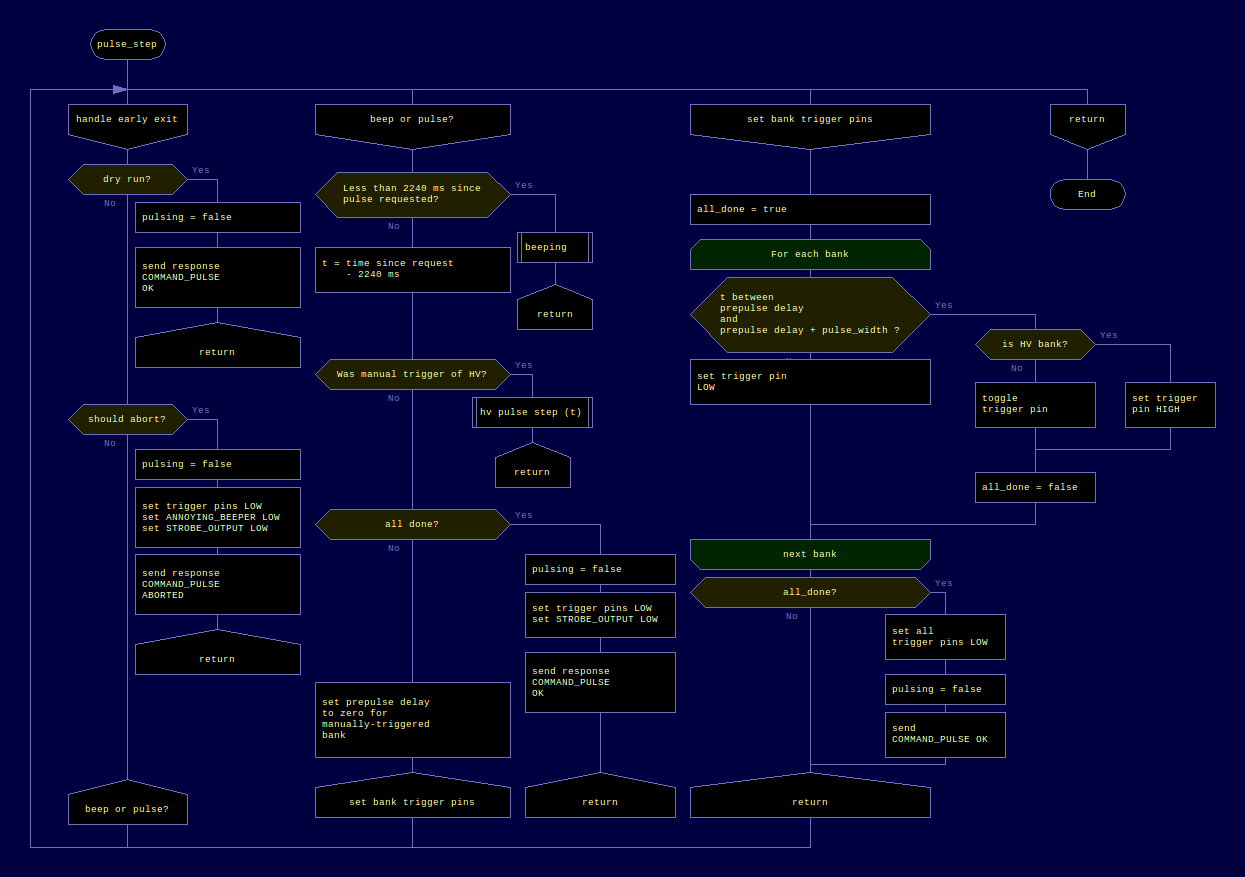
\includegraphics[width=400px]{pulse_step.png}
\caption{\label{fig:pulse_step} Pulse Step processing}
\end{figure}

\begin{figure}
  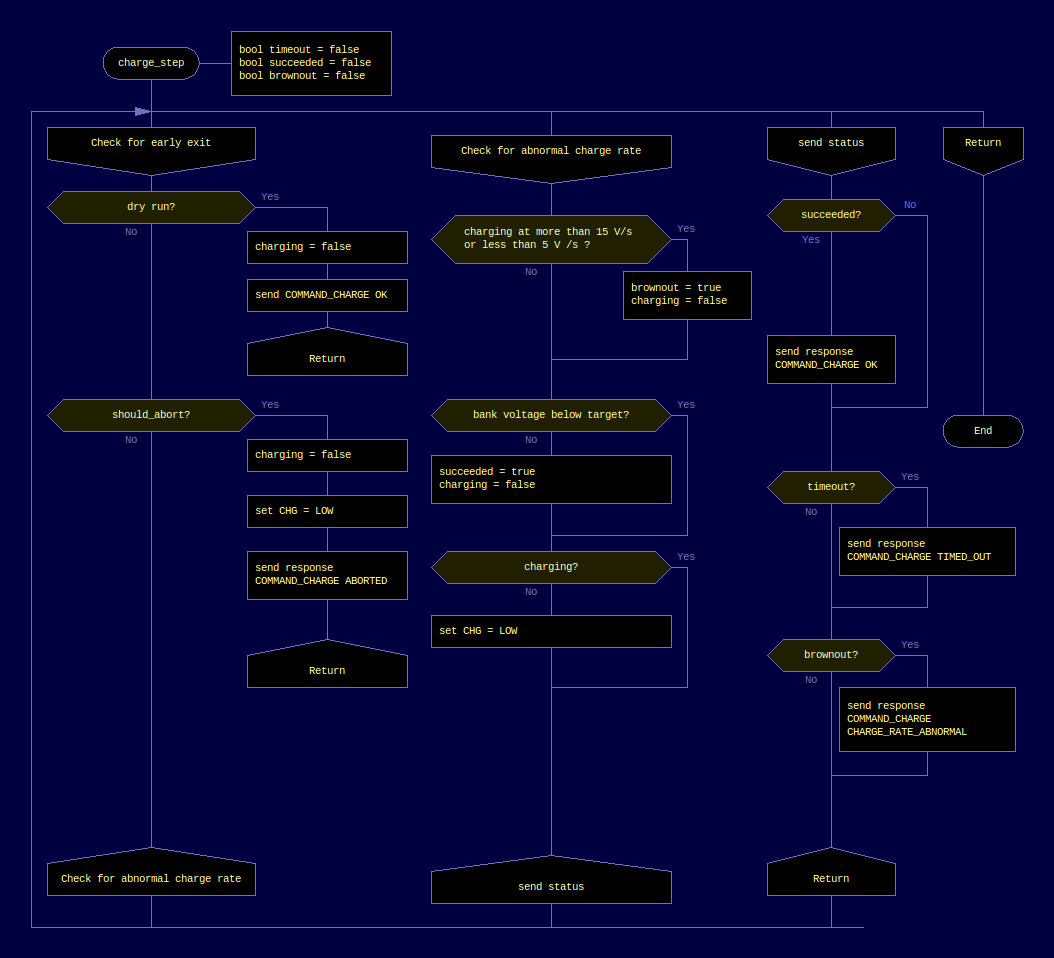
\includegraphics[width=400px]{charge_step.png}
\caption{\label{fig:charge_step} Charging step logic}
\end{figure}

\subsection{The Stepper Controller}

The stepper controller is an Arduino UNO; four pins and mosfets are used to switch an externally-supplied 12V to the poles of a stepper motor. The stepper motor accepts simple serial commands; e.g `F5' for forward 5 milimeters, or `R10' for 'Reverse 10 mm'.

\subsection{The IRC Server}

The IRC server is a raspberry pi running Linux. At present it has the fixed IP address 192.168.137.3.
The IRC server runs \textsc{ngircd}, an open-source IRC daemon. All user-facing software connects
to this IRC server. In this fashion, we can easily view and log all messages and commands being issued
or responded to by the various subsystems.

\subsection{The Agents}

Each important subsystem has its own IRC bot; there is a bankbot which translates commands and messages for the bank controller, a stepperbot for the steppers, and so on. There are also some utility IRC bots. The talkbot does text-to-speech translation, and the sequencebot can perform complex sequences of tasks,
including sending messages to the other bots.

The complete list of bots (Agents) presently in use is as follows:

\begin{itemize}
 \item{bankbot  : controls the cap bank and HV power supplies }
 \item{ipfsbot  : uploads files or directories to IPFS }
 \item{picobot  : controls the Picoscope 3405D oscilloscope }
 \item{rigolbot : controls the two DS10x4z oscilloscopes }
 \item{talkbot  : says things out loud - e.g countdowns }
 \item{robot    : runs complex sequences of commands }
\end{itemize}

\subsection{Using the System}
The \textsc{HexChat} application is set up to connect to the IRC server and become the system operator;
it then connects to the channel called \#system. The run\_bots.bat batch-file (linked to on the desktop) will
invoke all of the bots, which will then initialise themselves and connect to the same channel.

Sending any of the bots a message of the form ``BOTNAME: help'', e.g `bank: help', will cause
that bot to reply with a description of all the commands supported by that bot. To issue a command CMD, you can just type ``BOTNAME: CMD''.

\subsection{bankbot Command summary}

The bank control robot, bankbot, understands the following commands
\begin{verbatim}
  get <PARAMETER_NAME>
  set <PARAMETER_NAME> <VALUE>
  reset
  dry_run <1|0>
  pulse
  \abort
\end{verbatim}

PARAMETER\_NAME can be one of the following:
\begin{verbatim}
  pulse_width
  pulse_delay
  charge_enable
  charge_power
  hv_state
  hv_voltage
  bank_voltage
  switch_state
\end{verbatim}

The symbolic names True, False, On, and Off, may be used in place of 1 and 0.

\subsection{ipfsbot Command summary}

The ipfsbot understands only 'help' and 'publish'. The command 'publish' expects a path
as an argument and publishes all the files under that path to the IPFS filesystem. The
identifying hash value is returned as a URL enabling remote access to the published file.

\subsection{picobot Command summary}

The picoscope control robot, picobot, understands the following commands:

\small{
\begin{verbatim}
   start_capture  :  start_capture <TIMEOUT_MS> arms the picoscope for capture
   channel_config  : configures a chosen channel;
                       e.g  channel_config <NAME> <COUPLING> <VOLTAGE_RANGE>
   trig_threshold    sets the voltage threshold (in Volts used for triggering
   trig_channel   :  sets the channel used for triggering;  e.g "trig_channel A"  
   status         :  shows device configuration
   reset_scope    :  disconnects and reconnects scope
   write_data  :  write_data <PATH_PREFIX> writes the last data set to disk in HDF5 format  
   channel_names  :  'channel_names <NAME_1> <NAME_2> <NAME_3> <NAME_4> 
                      names the four device channels'
   help :  shows this useful message
\end{verbatim}
}

\subsection{rigolbot Command summary}

Rigolbot only supports DS10x4z devices at present. The commandset is:
\small{
  \begin{verbatim}
    channel_names :    channel_names <DEVICE_NAME> <NAME_1> <NAME_2> ... 
                         names the channels of the chosen scope
    add_device :       add_device <IP> <NAME>  adds the device at IP and names it NAME
                         (e.g add_device 192.168.137.10 pulse_scope
    remove_device :    remove_device <NAME> removes the named device
    status     :       shows information about connected Rigol scopes
    write_data :       write_data <PATH> writes the current screen contents of each rigol scope to <PATH>
    help :             shows this useful message
  \end{verbatim}
}

\subsection{talkbot Command summary}

Talkbot speaks any message sent to it. If you want talkbot to say 'Hello', you just
type 'say: Hello' in the \#system IRC channel.

\subsection{robot Command summary}

The sequencing robot, simply called robot, has a complicated commandset. This is because robot.py is essentially a Python interpreter connected to the IRC channel. The initial set
of commands is given in the file `macrosystem.py', and new commands can be defined at runtime.

The best way to learn to use the robot is to enter `robot: help' into the \#system IRC channel; nevertheless, a brief summary is as follows:

The robot has a few primitives built in:
\begin{itemize}
\item{help  -- shows a help message}
\item{emit(s) -- writes something to the channel, e.g emit("say: 5") }
\item{wait(s,timeout=1) waits to hear the string s from the IRC channel, or panics after timeout}
\item{process\_line(s) interprets a string}
\end{itemize}

The rules for process\_line are as follows:
\begin{verbatim}
lines starting with @ are executed
lines starting with ! are emitted to the channel
lines starting with # are treated as comments (ignored)
\end{verbatim}

New commands can be then defined by sending robot messages of the form
\begin{verbatim}
def function(arg1, arg2, ..) ->  python_code_line_1; python_code_line_2; ...
\end{verbatim}

In `macrosystem.py', this facility is used to build up some useful commands:

\tiny{
\begin{verbatim}
inputs = [
  'RUNDIR = r"c:\data\default_rundir"',
  'def setup_rigols() -> emit("rigol: add_device 192.168.137.10 rigol_1"); wait("Connected to rigol", 5)',
  'def charge_enable(s) -> emit("bank: set charge_enable " + s)',
  'def charge_power(s) -> emit("bank: set charge_power " +s)',
  'def countdown(n) -> [ (emit("say: "+str(d)), wait("OK", 5)) for d in range(n,0,-1) ]',
  'def setup() -> setup_rigols(); countdown(5); charge_power("on"); sleep(0.5); charge_enable("on")',
  'def shutdown() -> charge_power("off"); sleep(0.1); charge_enable("off"); emit("Shutdown complete")',
  'def charge(V) -> emit("bank: charge "+str(V)); wait("charge : OK, value = 0", 30)',
  'def start_capture() -> emit("picoscope: start_capture 5000")',
  'def pulse() -> emit("bank: pulse"); wait("pulse : OK, value = 0", 10)',
  'def collect_data(dir) -> emit("picoscope: write_data " + dir); emit("rigol: write_data " + dir)',
  'def shot(V, dir) -> charge(V); start_capture(); pulse(); sleep(1); collect_data(dir); sleep(10)',
  'def run_file(filename) -> state.seq = 1; [  process_line(line.strip()) for line in open(filename).readlines() ]'
]
\end{verbatim}
}

In the above you can also see that environment variables can be set and used as you might expect.


